\section{实验}

\subsection{设置与缓存合同}

模型为Meta-Llama-3.1-8B-Instruct，source为已审计task group-scale硬端点，逻辑码率2.1207557 bpp。开放layers 28--31的28个Linear、145,465,344个六维向量。五任务各使用512/256/31条互斥train/validation/audit，文本使用4096/128/64条长度4096的序列。实验固定8-way邻域、128/Linear bundle、层序和零文本预算，不扫描seed、bundle、阈值、LR或group。只用本机GPU5单卡，耗时3.695小时、峰值25.285GiB。

Task cache的32例parity覆盖五任务、长度11--163和continuation起点7--133；最大choice-score误差$1.1444\times10^{-5}$，argmax 32/32一致。Text cache包含16,777,216个next-token位置；8条覆盖首尾的parity与同batch完整HF transformer路径最大和平均CE误差均为0。完整4096行参与目标，8行只用于双路径数值校验。

\subsection{任务收益与文本可行性}

\begin{figure}[t]
\centering
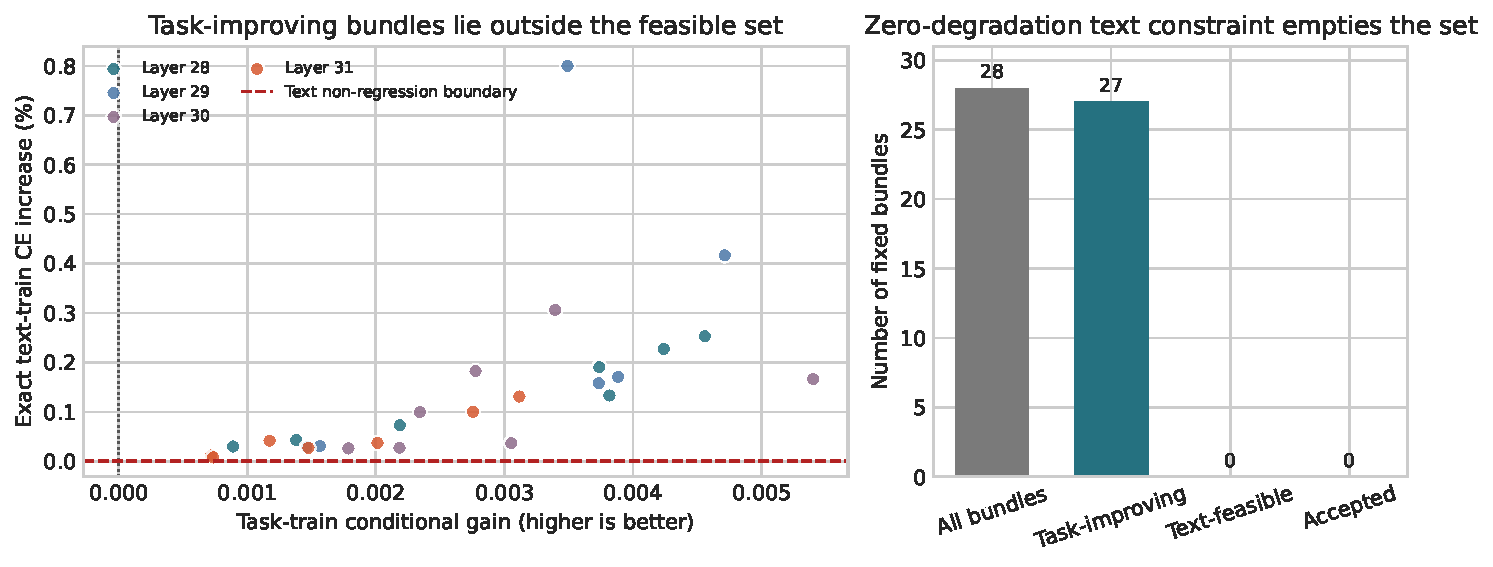
\includegraphics[width=\linewidth]{../img/v14_text_feasibility.pdf}
\caption{左：进入文本计算的27个task-improving固定bundle全部位于零退化边界之外；layer-29 Q projection因task gain为负，按合同未计算文本CE、未画入散点。右：28个动作经task与text可行性过滤后没有可接受bundle。}
\label{fig:v14}
\end{figure}

\begin{table}[t]
\centering
\small
\caption{每层固定动作的task收益与text可行性。}
\begin{tabular}{lrrrr}
\toprule
层 & Task+ & Text可行 & 最大task gain & 最小text增幅\\
\midrule
28 & 7 & 0 & 0.004559 & $+0.02976\%$\\
29 & 6 & 0 & 0.004714 & $+0.02896\%$\\
30 & 7 & 0 & 0.005403 & $+0.02603\%$\\
31 & 7 & 0 & 0.003117 & $+0.00785\%$\\
\bottomrule
\end{tabular}
\end{table}

28个bundle中27个严格降低task-train combined loss，任务收益并不稀缺。唯一负项为layer-29 Q projection，gain为$-6.32\times10^{-5}$，按合同不计算文本CE。Source text CE为2.1035536536；27个被评估候选全部上升，最小绝对增量0.000165183（$+0.0078526\%$），最大0.016824409（$+0.7998089\%$）。四层可行集均为空。

\subsection{正控制、终态与比较边界}

四层曲率--即时block MSE Spearman分别为0.9643、0.3571、0.5714、0.7143；局部曲率在部分层能预测即时失真，但不能决定双目标可行性。四层均保持source，accepted bundles/switches为0。Launcher写\texttt{text\_constrained\_gain\_rejected}并正常退出0。

因为没有候选endpoint，task/text validation为null，audit未访问，checkpoint未写，formal test未使用。V14没有新PPL或准确率，不能复用source历史指标声称超过QTIP或GSQ。最小$+0.00785\%$虽小，仍违反预注册零预算。零预算是无交易方向的机制探针而非现实部署唯一阈值；事后扫描非零容忍度会改变科学问题，必须作为新的预注册实验处理。

\subsection{机制解释与局限}

27个点均落在$\Delta L_{\rm task}<0,\Delta L_{\rm text}>0$象限。过滤规则只能从已有动作选择，不能创造双非正方向；剩余问题属于action space而非对同一动作集合重排序。可能的新动作包括有原理的可撤销子结构或跨Linear补偿坐标，但非线性交互使独立一阶相加仍不充分。任何新动作$A$必须先在train上证明$G_{\rm task}(A)>0$且$T(S\cup A)\le T(S)$，之后才允许访问validation/audit。

实验只覆盖一个8B Instruct模型最后四层和固定top-128粒度，不能外推为所有assignment全局无解。Teacher目标是固定top-32分布上的精确full-vocab CE，不是原始dense全分布或生成质量。零退化train是必要性探针而非部署证书。128GiB宿主缓存与3.695小时成本也限制该检验作为通用训练算法的实用性。
